\begin{document}
\section{Preseason/Summer Practices}
\begin{comment}
 format for the practice notes entry.   \practicenotes{Date and time}{Type (practice/league meet/meeting}{People (alphabetical please}{Boxes: Begin with team or task\\\\ notes\\\\Written by: who wrote it. \newBox between boxes}
\end{comment}

\practicenotes{5/11/19 3:00pm - 9:00pm}{Summer Practice}{Ori}{
    Design and CAD\\\\
    Ori designed and CADed a custom parallel plate drivetrain. It is one of the possible drivetrains to be used in the upcoming season. It would have a total cost of \$375.95.\\\\
    Written by: Ori
}
    
\practicenotes{6/17/19 6:00pm - 10:00pm}{Summer Practice}{Ori}{
    Design and CAD\\\\ 
    Ori CADed another drivetrain. This one is fully made of goBilda and is cantilevered. It would be very modular and easy to build on. Not only is it a viable option for next year's robot, it also helped with understanding and practicing with goBilda structure. The total cost would be \$359.54.\\\\
    Written by: Ori
}
%6-10
    
\practicenotes{6/23/19 6:00pm - 11:00pm}{Summer Practice}{Ori}{
    Design and CAD\\\\
    Ori CADed a different drivetrain that uses boxtube as the sides that support the wheels. It is also cantilevered and uses a mix of custom made parts and goBilda structure. It has a total cost of \$289.73.\\\\
    Written by: Ori
}
%6-11

\practicenotes{6/24/19 4:00pm - 7:00pm}{Summer Practice}{Ori}{
    Driver Control\\\\
    \wrapCap{r}{Images/unitysimulation.png}{.5}{The Unity driving simulation}
    Ori made a simulation in Unity for the use of testing different kinds of mecanum drives. The two different driving methods that were created were field-centric and robot-centric. In the simulation, a chassis and field model were imported and scaled to the correct sizes. Ori also made sure that the speed of the robot would be accurate so that driving the robot would be as accurate as possible. An Xbox controller is connected to the computer and then the robot can be controlled. Robot-centric drive is based on the position of the robot. Moving the left joystick upward would result in the bot moving in the direction it is facing. Field-centric means that moving the left joystick upward would result in the bot moving in the direction the driver is facing (the robot has to be told which direction that is before starting), regardless of which direction the robot is currently facing.\\\\
    Written by: Ori
    \newBox
    Programming\\\\
    Ori started working on the math for a robot-centric drive for tele-op. He coded it in Android Studio. Since he didn't have access to phones to test the code, he imported the math and logic into Unity to get the motor power values. The code wasn't ideal since the max motor power value would be about $\frac{\sqrt{2}}{2}$, instead of 1. He then went through the math and other mecanum drive code examples to fix it. Right now, it can't be tested since he doesn't have access to the necessary electronics.\\\\
    Written by: Ori
}

\practicenotes{6/26/19 3:00pm - 10:00pm}{Summer Practice}{Ori}{
    Programming\\\\
    \textit{Finding suitable complex motion options:} One issue that Ori had on his robotics team last year was getting the PID and gyro to work for autonomous. This took a lot of time, and finally broke before the state competition, where some of the gyro turns wouldn't work. One way to get a heads up for next year is to figure out if there are any accessible libraries or tutorials to have better motion. The first option is Pure Pursuit, which was made by FTC team 11115 Gluten Free. This consists of a basic library for path-making and a debugger that maps out the motion of the robot. Gluten Free also made some tutorials for setting up the basic code for Pure Pursuit. How it works is you set up a path made of lines, and then set a radius around the center of the robot. The circle then intersects with the path, and that then creates a vector that then sets the direction of the given velocity. It goes through the path and makes curves around the given turns to smooth motion, getting rid of the need for straight paths and turns. The second option is Road Runner, which is an open source motion profiling library. The library contains functions to create splines, PID tuning code, motion profiling for driving and lifts, complex strafes, and other complex holonomic drive code.\\\\

    \textit{Setting up Road Runner:} Ori spent the day setting up and figuring out how Road Runner works. Online, there is a Road Runner tour that shows the basics of how it works and what the different functions can do. It also gives explanations for how the PID works and how the PID tuning op-modes work. The makers of Road Runner also made Road Runner Quickstart, which has example code for most of their functions. There is also a plugin that is made for visualizing motion splines on a field with a tab for graph of the position, velocity, and acceleration functions. These splines then can be created in an op-mode and the robot will follow the path with the given max velocity and acceleration values. Nothing can be tested until Ori retrieves a robot from last year from Sarah to get the PID set up and start testing some code.\\\\
    Written by: Ori
}

\img{Images/pathdesigner.png}{An example of spline creation in the path designer program for Road Runner}{1}
\img{Images/pathdesignergraph.png}{The trajectory graph of the created spline}{1}
\newpage
\practicenotes{6/27/19 2:00pm - 10:00pm}{Summer Practice}{Ori}{
    Programming\\\\
    \textit{Setting up Pure Pursuit:} Ori worked on setting up the Pure Pursuit debugger to work on IntelliJ to run the motion code without an actual robot. He then followed the Pure Pursuit tutorials to get some simplistic functionality working. The code works by getting a given array of points to make a path of lines in between the points. Then, the circle around the center of the robot intersects with the path to make curves. The code makes it so that the robot follows the given path, but isn't on a strict line. This means that if the wheels slip on the field or the robot comes in contact with another thing, it still follows the path without any error in it's ending state. One issue that is still not fixed is at the end of a path, the robot orbits around it.\\\\
    Written by: Ori
}
%2-10

\img{Images/glutenfreemotion.png}{The path the robot is told to take is the blue line. The blue circle on that line is the point where the robot is going to next, which is always a certain distance ahead of the robot. The dotted line is the actual path the robot takes.}{1}

\newpage
\meetingnotes{7/1/19 3:00pm - 6:00pm}{Meeting}{Julia, Michael, Oliver, Ori, Rachel, Sarah}{

    Summer practice & The team decided that we wanted to spend time over the summer to get prepared for next year. Although the challenge is released in September, there is still stuff that we can do. Some things include preliminary design and teaching each other skills such as CAD, programming, and using Overleaf, the program we use to write our Engineering Notebook. Even though we could do these things by ourselves, having planned meetings would help with organization and make everything easier. These summer practices would also be used to make a beginning drivetrain and get some basic motion profiling to work so that it would be easy to use during the season. We planned to meet at either Michael's or Ori's house every Monday.\\\\
    
    Agile project management & We decided that it would be effective to use a more agile model of project development this season, since in our experience the ideas we have for the challenge are changing constantly. We will have two week sprints (since league meets are every two weeks, this will help us prepare to have a functional robot at each meet), and a meeting at the beginning of every two weeks to reflect on what happened in that sprint and what will need to get done in the upcoming sprint.\\\\
    
    CAD & Out of everyone currently on the team, Ori is the only one proficient in CAD, and the rest of us would like to learn. We plan to participate in the Valor CAD Challenge by team 6800 Valor. 6800 will release a fake challenge, and participants must CAD a robot for the challenge in five days, which will also need a page for strategy and how the robot will work. This will help us learn to use CAD, design parts of a robot, and practice documentation on how the robot works. \\\\
    
    Notebook & Rachel is the most competent at using Overleaf and writes the custom commands that make our notebook easier to use. Ori and Rachel both used Overleaf last year, and the rest of the team will eventually learn some basics as well as how to use the custom commands to write entries. Rachel has a custom command for engineering entries that formats them into a table, which her team used last year, but we decided on a format where different teams will each have a box in a table where they can record what they did as well as add pictures. This format wastes less space and makes it easier to organize the entry, since the categories will be broad groups instead of specific tasks. It will also make it easier to know who worked on what. The teams will change based on what we need to focus on. We also decided on a format for our meeting entries, which is a simple table with two columns that have the topic and notes from each part of the meeting.\\
}

\practicenotes{7/1/19 5:00pm - 7:00pm}{Practice}{Ori}{
    Programming \\\\
    \textit{Robot-centric mecanum code:} After the meeting, Sarah gave Ori the 10565 robot from the previous season, which also included the phones and controllers. Now that he had access to the phones, he could actually test the code he had, which turned out to not work. He then revisited the math which he had and tried fixing it again. This still didn't exactly work because the angle created by the trigonometry wasn't aligned with the actual angle and adding the different aspects to get the power were also off. Another issue that came up is that the scaling of the joysticks wasn't working, so the power would either be zero or one. Scaling the joysticks mean that the output value follows a cubic equation, so the values aren't linear. This makes it so there is more room for precise movement. The reason this happened is because the code would normalize the power so that it would stay at a range from -1 to 1. To do this, we need to find the max power and then divide the power given by the equation by the max power. The max power needs to be set to a number higher than zero because if not, we would be dividing by zero. It was originally set at one, but this meant that if the power given was less than one, the max power would still be one.\\\\
    Written by: Ori
}

\practicenotes{7/2/19 2:00pm - 6:00pm}{Summer Practice}{Ori}{
    Programming\\\\
    Ori started playing around with Road Runner and using the tests\\\\
    Written by: Ori
}

\practicenotes{7/3/19 5:00pm - 11:00pm}{Summer Practice}{Ori}{
    Building\\\\
    \textit{Making a better goBilda drivetrain:} During the meeting on Monday, the team decided to go for the goBilda drivetrain. Since the drivetrain Ori CADed wasn't ideal and was expensive, he decided to CAD another one that would be cheaper and better. He also planned on making it based off of parts that the goBilda FTC kit has since there was talk of getting one over the summer. There were many ways to make it cheaper. The first way he made it cheaper was by designing some 3d-printed ball bearing pillow blocks instead of buying them from goBilda. For the necessary 8 pillow blocks, it would cost \$47.92. Making our own pillow blocks meant that we could use cheaper ball bearings and eliminate that cost. The other reason it was so expensive was that the original goBilda drivetrain used 4 pieces of half channel, which costs \$51.96. To reduce the cost, full channel was applied instead. The downside to this is that they are larger, making it harder to fit in the box. Because of the full channel, the overall robot's width was at 17.8 inches, not leaving enough room for the screws for the mecanum wheels. One way that Ori fixed this is by moving the pillow blocks to the inside of the channel. This meant that the outsides had more room so the wheels could be closer to the channel. One side effect of this was that the belt pulleys attached to the motors were further away, and the shaft collars to keep the pulley in place wouldn't be able to fit on the axle. To fix this issue, the pulleys for the motors would need to be press-fitted so they won't fall off. Now the drivetrain has a width of 17.5 inches, so it is in the box and has room for screws and other possible parts.\\\\
    \textit{Press-fitting pulleys:} In order for the pulleys to go on to the axle and stay there, the hex hole would need to be the right size. In order to find it, different hex hole sizes were used. Instead of printing pulleys, which would take hours to do, simple cylinders that are 5mm tall were used. These only take 16 minutes to print, making it easier to test. Ori first started with 3d printing the right size, just to see what needed to be changed. The pulley fit on the motor, but it didn't stay in place. He then made one where the hexagon's circumscribed diameter was 0.5mm less than the original. This was an overshoot, but it made it easier to cut down on which was actually correct. After it was printed, it wouldn't fit, so Ori went on to go halfway, and made one with a diameter of 4.75mm. This time it eventually fit on the axle, but with a lot of force, which wasn't ideal. Again, he went in between that and the regular diameter and made one with a diameter of 4.875mm. This test turned out to be ideal, and will be used for the pulleys.\\\\
    Written by: Ori
    \newBox
    
    
    Design and CAD\\\\
    Throughout the day, Ori 3d-printed the belt pulleys that would attach to the wheel axles. These pulleys all took 2 hours long, and since all the drivetrains used the same ones, it was better to print them sooner than later.\\\\
    Written by: Ori
    %add pictures of the pulleys
    %add pictures
}
\infoBox{Mecanum Wheels}{}

\practicenotes{6/24/19 3:00pm - 2:00am}{Summer Practice}{Ori}{
    Design and CAD\\\\
    \wrapCap{r}{Images/forwardDeadWheelPod}{.5}{Forward Odometry Pod}
    Because the team is planning on using mecanum wheels, they planned on using odometry wheels, also known as dead wheels, to know the position of the robot more accurately. These wheels are attached to their own encoders instead of the ones on the motors driving the wheels. The team plans on using these because mecanum wheels can have quite a bit of slippage, which leads to a less accurate position determined by the encoders. There are two different pods needed, two to measure the distance going forwards and backwards, and another to measure the sideways distance. 
    \wrap{l}{Images/sidewaysDeadWheelPod}{.3}
    Ori then created two pods that would be able to fit in between the mecanum wheels to waste as little space as possible. Most of the pods are 3d-printed, aside from the omni-wheels, axles, ball bearings, and hubs.
    
    Since the odometry wheel pods are fragile and need to be protected, Ori then made plates that are on the outside of the pods to cover them. These are also useful to help protect the mecanum wheels since it stops other robots from hitting them from the inside. They might also be used to put the team number and alliance marker on.\\\\
    Written by: Ori
}
\img{Images/deadWheelPods.png}{Odometry pods attached to the drivetrain}{1}
\xvspace
\infoBox{Odometry Pods}{Ori write something here and maybe pictures too}
\newpage
\practicenotes{7/8/19 3:30pm - 6:30pm}{Meeting}{Josh, Michael, Oliver, Ori, Sarah}{
    CAD and Design\\\\
    Since part of the team is competing in the Valor CAD Challenge and people want to learn CAD, the team needed to learn CAD. At this time, Ori was the only one with proficient CADing knowledge for FTC. Oliver understands how to CAD, but has never CADed for a robot. Ori spent the practice getting Michael and Sarah familiarized with basic CAD skills, like how to created sketches and extruding them to create parts. He also told them basic assembly skills, which was mostly made of showing them rigid joints. They were then told to create specific parts. Sarah was given the task to create a Tetrix L-bracket while Michael was given the task to create an old part from last year.\\\\
    Written by: Ori
    \newBox
    Programming\\\\
    Started to work on improving vision software that my team (10565) used last year. I worked on posterization, which is where the phone has an image and turns the colors into basic colors. I changed the posterization to use YUV color space instead of RGB color space. YUV color space has 1 luminance component and 2 color components as opposed to the 3 color components of RGB. This should make it easier to distinguish different colors, even at low brightness and make it easier to distinguish different shades of grey. \\\\
    Written by: Josh
    \newBox
    Logistics\\\\
    Fundraising: After most people left, Ori and Oliver talked a little bit about getting sponsors and fundraising money for Wilson Robotics. They looked at some local businesses for possible sponsors. One place they looked at was Dairy Hill, a local ice cream shop. They also looked at Pizzicato, which has a fundraising campaign called Dough for Dollars.\\\\
    Written by: Ori
}

\practicenotes{7/16/19 4:00pm - 7:00pm}{Summer Practice}{Josh, Michael, Oliver, Ori, Rachel}{
    CAD and Design\\\\
    We talked about potential design ideas for the Valor CAD Challenge and discussed their game manual and the specifics of the challenge. The challenge consists of shooting frisbees through hoops, pressing beacons, and hanging from the hoops among other ways of scoring points. Jaren (Ori's brother and FTC alum) taught everyone (mostly Oliver) how to constrain things in CAD. We have 2 teams worth of people, and considered a big-arm design and a turret-like design. The two teams are using different drive trains: octocanum drive, mechanum drive, 6-wheel drive, etc. Jaren is leading one team and is going to use an octocanum drive and make a turret to shoot the frisbees. The turret will use a differential gearbox to turn. Ori is leading the second team\\\\
    Written by: Rachel
    \newBox
    Programming\\\\
    I decided to not use YUV color space because the 2 color components alter the color in non-intuitive ways and the actual color changes with the luminance value. Instead I worked on posterizing using the HSL color space and included more colors. The posterization is overall pretty good but trends toward red in bright spots.\\\\
    Written by: Josh
    \newBox
    Notebook\\\\
    \wrap{r}{Images/overleafPractice.png}{.4}
    I wanted to finish formatting the daily practice entries. Last year, I used a format with a table that looks similar to our notes for meetings this year. This year, I wanted to organize the entries by topic/team (ie Programming, Design, or Building) instead of by task (ie "Design a chassis"). I had to find a new table environment called longtabu, which combines elements of tabu, which makes the dimensions easier to manage for the table I want to make, and longtable, which allows the table to extend onto the next page.\\\\
    Written by: Rachel
}

\vfuzz=1pt
\needspace{2\baselineskip}

\vspaceleft=\textheight
\advance\vspaceleft by -\pagetotal
    
\xleaders\vbox to \vspaceleft{%
    \vspace{1em}\hspace{2pt}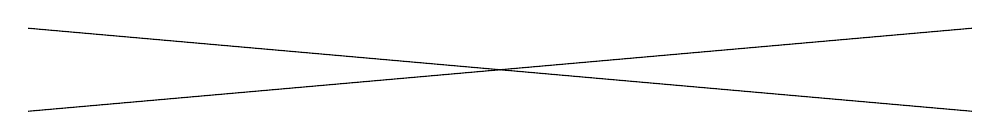
\begin{tikzpicture}%
        \draw (4pt,1em) -- (\textwidth,\vspaceleft-2em);%
        \draw (\textwidth,1em) -- (4pt,\vspaceleft-2em);%
    \end{tikzpicture}\vspace{1em}%
}\vfill
\clearpage
\newpage

\practicenotes{7/22/19 3:30pm - 9:00pm}{Summer Practice}{Josh, Julia, Oliver, Rachel, Sarah}{
    CAD and Design\\\\
    Julia is learning how to CAD in OnShape. Oliver is becoming more proficient in Fusion360 with help from Jaren (Ori's brother). He CADed an intake for the Valor CAD Challenge. Sarah is practicing CADing in OnShape, since she has a little experience with SolidWorks but not with OnShape.\\\\
    Written by: Rachel
    \newBox
    Notebook\\\\
    I'm working on getting rid of the errors in Overleaf. They don't prevent the notebook from compiling, but I want to understand why they occur and what I should change. Started the day with 102 errors and ended with 84. I think most of them are related to the custom commands since they occur often, but even with the errors the notebook still formats the way I want it to.\\\\
    Written by: Rachel
}
\practicenotes{8/5/19 3:30pm - 5:30pm}{Summer Practice}{Josh, Michael, Ori, Sarah}{
    Programming\\\\
    Josh worked on some vision stuff for recognizing stuff. We think we will be using Vuforia, as opposed to Josh's custom blob detection algorithm he developed last year.\\\\
    Written by: Rachel
    \newBox
    CAD and Design\\\\
    Ori continued working on the robot that had been CADed for the Valor CAD Challenge.\\\\
    Written by: Rachel
}

\practicenotes{8/5/19 3:30pm - 10:00pm}{Summer Practice}{Julia, Oliver, Ori, Rachel, Sarah}{
    Notebook\\\\
    The first thing we did today was create a google account that everybody on the team can access. This new account allows us all to access the notebook and be able to work on it. Rachel helped the team  learn how to create entries in the notebook. Rachel also continued to debug some of the errors.\\\\
    Written by: Julia
}
\practicenotes{8/12/19 3:30pm - 9:00pm}{Summer Practice}{Julia, Oliver, Ori, Rachel, Sarah}{
    Logistics and Marketing\\\\
    Oliver brought the coat that he had already ordered to the meeting so we could all figure out about what size of coat we would need for the season. Oliver also worked on writing a sponsor letter to Pizzicato that could be adjust to work for other places.\\\\
    Written by: Rachel
    \newBox
    Building\\\\
    We worked on disassembling the old robot so that we can take inventory of what parts we have and need. Ori also worked with some people to create a slide component for linear movement that we hope to use during the season.\\\\
    Written by: Rachel
}    
%testing
\infoBox{title}{words}

\newpage
\meetingnotes{8/19/19 3:30pm - 5:30pm}{Meeting}{Josh, Julia, Michael, Oliver, Ori, Rachel, Sarah}{
    Goals and expectations & When we formed the team, we decided that we wanted to be very ambitious and competitive this year. We will have work time that is in addition to practices with the other Wilson teams so that we can all put in the time that we want and give ourselves the opportunity to be successful. We all can work independently, and when we add rookies to the team we will look for people who have similar mindsets. We established that the role of our coaches will be as an oversight role and to make sure that we are sticking close to the timeline that we will set for ourselves, and that everyone is responsible for what they say they will contribute.\\\\
    Rules & We decided that for all building, at least two people should be working on any larger component. This will allow us to continue working efficiently if one person is absent because the second person will know what is going on. We also decided that every two weeks, someone other than the two main coders will "proofread" the code. This will allow everyone to have a basic understanding of what the code does, and the coders will have to be able to explain their code.\\\\
    Structure and decision-making & For any large design decisions, we will have a team vote if there is a disagreement. For smaller design decisions that are easier to prototype, both/all ideas will be prototyped so that the team can decide which one is the best. Teams working on specific components of the robot can make design decisions without consulting the rest of the team, but they should consult with anyone else who is working on the same part or a related part. This overall structure allows the team to be involved in all main decisions so that everyone has the chance to contribute ideas, and nobody will be left out of the design process. It also allows individuals/small groups to make small decisions without having to consult the team, which makes our building process more efficient. All changes and decisions made should be documented in the notebook so that the rest of the team is up to date.\\\\
    Logistics and schedule & This year, Wilson Robotics Club is limiting the amount of practice time and significantly shortening it from what it was last year. The whole club will only be practicing on Wednesdays and Fridays for 3 hours each, which means we would only get 6 hours of work time per week. We want to be able to work more than this and will be adding 6 hour practices on Mondays, and maybe an optional weekend practice if there is a lot of work to do. Mondays will be spent as mostly build time. We will have a team meeting every Wednesday to check in, and every two weeks we will have a large meeting to assess our work timeline and see what needs to be done. Wednesdays will also be time for coding, and both Wednesdays and Fridays some of the team will dedicate time to helping/interacting with other Wilson teams.
}
\practicenotes{8/19/19 5:30pm - 8:30pm}{Summer Practice}{Josh, Julia, Michael, Oliver, Ori, Rachel, Sarah}{
    Building\\\\
    We received the parts that we ordered to start building a drivetrain, other than the mecanum wheels. We finished taking apart last year's robot and started building the new drivetrain out of goBilda parts. To complete the drivetrain, we are waiting for the mecanum wheels as well as the omni wheels that we will use in the odometry pods.\\\\
    Written by: Rachel
}
\practicenotes{8/20/19 3:30pm - 9:00pm}{Summer Practice}{Ori}{
    Building\\\\
    We finished building the chassis and it works. We realized that Amazon sent us wheels with bushings instead of bearings even though they had the order code for the ones with the bearings, but the bushing wheels work fine for now.\\\\
    Written by: Rachel
}

\end{document}